%\documentclass{article}
%\documentclass[10pt,twocolumn]{IEEEtran}
%\usepackage[a4paper, margin=1in]{geometry}%lmargin=1in, rmargin=1in, tmargin=1in, bmargin=1in]{geometry}
%\usepackage{algorithm}
%\usepackage{algpseudocode}
%\usepackage{svg}
%\usepackage{xcolor}
%\usepackage{multirow}
%\usepackage{booktabs}
%\bibliographystyle{plain}
%\usepackage{float}
%\usepackage{boldline}
%\usepackage{pbox}
%\usepackage{tabularx}
%\usepackage{graphicx}
%\usepackage{amsmath}
%\usepackage{amsfonts}

%\begin{document}

\section{Experimental Results}
\label{sec:exp}
\iffalse
%\iffalse
This section presents the results of reducing modulo multiplier
circuits used in cryptography using our implementation. The
experiments are performed on a 3.5GHz Intel 
Core\textsuperscript{TM} i7-4770K Quad-Core CPU with 32 GB of RAM. There are
two architectures that implement these multipliers, namely Mastrovito
and Montgomery. 
Mastrovito multipliers compute $Z = A\times B \pmod{
  P}$
%take $\{A,B\} =
%\{a_0,a_1,\dots,a_{k-1},b_0,b_1,\dots,b_{k-1}\}$ as $k$-bit inputs and
%produce $Z = \{z_0,z_1,\dots,z_{k-1}\}$ as $k$-bit output. The multiplier
%performs $Z = A \times B \pmod{P}$, 
where $P$ is a given primitive polynomial for the datapath size
$k$. 
%The procedure 
%involves computing the product $S=A\times B$ using an array multiplier
%and then reducing it $\pmod{P}$ to obtain $Z$. We perform experiments
%on \textit{flattened} netlists of these circuits.  
Montgomery multipliers perform fast modular multiplication without
explicitly performing the reduction $\pmod{P}$. 
%They are more
%efficient than the Mastrovito multipliers when several modulo
%multiplications are required as in the case of exponentiation in
%cryptosystems. 
Fig.~\ref{montfig} shows the structure of a Montgomery
multiplier. Each MR block computes $A\cdot B\cdot R^{-1}$, where $R$
is selected as a power of a base ($\alpha^{k}$). We denote the leftmost
two blocks as Block A (upper) and B (lower), the middle block as Block
C and the output block as Block D. We have presented results for GBR
on both \textit{flattened} and \textit{hierarchical} netlists of these
multipliers. 

\begin{figure}[H]
  \centering
  %\def\svgwidth{340pt}
  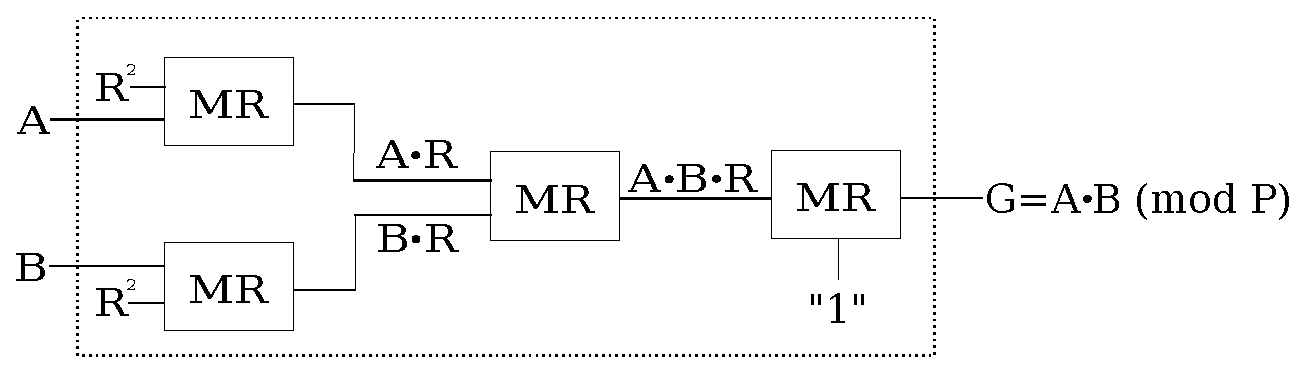
\includegraphics[scale=0.34]{new_mmcircuit}
  \caption{Montgomery multiplication}
  \label{montfig}
  \end{figure}

 
Table~\ref{masmm} provides the statistics on the time, ZBDD size, and
savings in the number of monomial cancellations achieved by our
approach as compared to classical symbolic algebra methods, for
Mastrovito multiplier circuits. The time reported is the total time
required to perform the reduction, $z_i \xrightarrow{G}_+ r_i$, for
all $i = 0,\dots,k-1$. The columns 
\textit{F4}, \textit{PB}, and \textit{ZR} represent the time taken in
seconds by F4 style reduction, PolyBori (version 0.8.3) and our
implementation respectively. \textit{MN} represents the maximum size
of any ZBDD encountered during reduction of any output-bit, while
\textit{MR} represents the maximum size of the ZBDD among all final
remainders $r_i$. \textit{CS} represents the
number of iterations saved during reduction due to our implicit
method. PolyBori throws a segmentation fault for the multiplier with
$k = 571$ which is depicted as \textit{CR} in the table. Our approach
is orders of magnitude faster than both \textit{F4} and \textit{PB}. 

Table~\ref{montmm} provides the same statistics for \textit{flattened}
Montgomery multipliers. The data for \textit{MN} and \textit{CS}
columns in  case of  $k=571$ could not be procured as both these
operations require traversal along ZBDDs (using the procedure {\tt
  Cudd\_zddDagSize()} and {\tt Cudd\_zddNextPath}). As there is a huge
number of large-sized intermediate ZBDDs produced during this
reduction, traversing along each path of every ZBDD is
infeasible. Also, the reduction times for $k=283$ is inordinate when
compared to other datapath sizes, which is purely due to  the
structure of the circuit.  


%The reduction times for $k=283$ is inrodindate when compared to other datapath sizes, which is purely due to the structure of this circuit.

%Table~\ref{montblockmm} and~\ref{montblockstats} depicts the comparison of time, ZBDD size, and monomial savings across \textit{Montgomery} Flat multiplier circuits with different field sizes. \textit{F4}(F4 style abstraction)*reference to Tim's paper*, \textit{PB}(PolyBori), and \textit{ZR}(ZBDD Reductions) represents the time in seconds for the respective implementations. \textit{MN}(Max Nodes) represents the maximum number of ZBDD size encountered, while \textit{MR}(Max Remainder) represent the maximum size for any remainder after the reductions. \textit{CS}(Cancellation Savings) signifies the total amount of monomial savings with our implementation.

%Table~\ref{montblockmm} depicts the comparison of ZBDD max size, remainders, and monomial savings across \textit{Montgomery} Block multiplier circuits with different block sizes, given different field sizes. For a given Block and field size, \textit{MN}(Max Nodes) represents the maximum number of ZBDD size encountered, while \textit{MR}(Max Remainder) represents the maximum size for any remainder while doing reductions with our implementation. \textit{CS}(cancellation savings) signifies the total amount of monomial savings with our implementation.

Table \ref{montblockmm} present the
statistics for hierarchical Montgomery multipliers for the blocks A,
B, C, and D. The experiment first reduces the outputs of a block
modulo the gates of that block, and then reduces the primary outputs
modulo these four sets of remainders (ZBDDs), thus exploiting the
hierarchy of these circuits. Table~\ref{montblockmm} shows the time
for reduction of each block and the time for reducing the primary
outputs across the four levels. The  time for reducing the primary
outputs across  levels in case of F4 implementation is $<$1 second,
and is not explicitly mentioned in the table. The row labeled
\textit{Total} presents the sum of time of reduction across levels and
the maximum reduction time for each block (as the reductions for the
four levels are independent of each other and are done in
parallel). The datapath sizes of these circuits correspond to
NIST-specification in cryptography with $k = 163,\dots,571$ bits.

%\par The reduction time presented in this section is obtained by reducing each output bit sequentially. These runtimes can be further improved by running these reductions in parallel.

%% The reduction times for small integer arithmetic array multipliers are
%% presented in Table \ref{intmm}. There is an 8x increase in time when
%% moving from $n-1$ datapath size to $n$-bits, which is an exponential
%% increase. Performing detailed analysis of a 7x7 multiplier reveals
%% that, when reducing the $z_{13}$ bit (MSB) and $z_{12}$ bit of this
%% circuit, the maximum number of monomials encountered are 429,889 and
%% 897,955. Of these, 269,120 monomials are {\it common to both output
%%   bits}. This implies that integer multipliers require a word-level
%% decision procedure, as given in \cite{ciesielski:dac2015}
%% \cite{rolf:date16}, that account for the cancellation of these
%% monomials across multiple bits in one word-level expression. Our
%% results show that bit-level techniques cannot efficiently verify
%% integer arithmetic circuits, but are very efficient for finite-field
%% arithmetic circuits.    
%\fi


%\iffalse
%%%%%%%%%%%%%%%% Mas Multipliers %%%%%%%%%%%%%%%%%%%
\iffalse
\begin{table}[H]
\centering
%\caption{Mastrovito Multipliers (Time in seconds, \# of nodes, \# of redundant monomials in $k$)  (K = $10^3$, M = $10^6$)}
\caption{Mastrovito Multipliers (Time in seconds)  TO = 3 days, (P):Parallelization, (WP):Without Parallelization}
\label{masmm}
\begin{tabular}{| c | c | c | c | c | c | c |} \hline
%\multirow{2}{*}{\textbf{Input}} & \multirow{2}{*}{\textbf{Abstraction}} & \multicolumn{3}{ c |}{\textbf{ZBDD reduction(ZR)}}  &  \multirow{2}{*}{\textbf{ZR improved}}\\ \cline{3-5}
% & &Building ZBDDs&Reduction&Total&\\ \hline
\textbf{Datapath(k)}&\textbf{\# of Gates} & \textbf{F4} &\textbf{\#T}&\textbf{CX(P)} & \textbf{PB(WP)} & \textbf{ZR(WP)}\\ \hline
163 &153K& 1,443 &30& 110 &70& 9  \\ \hline 
233 &167K& 1,913 &30&169 &105& 9 \\ \hline
283 &399K& 11,116 &30&496&316& 37 \\ \hline
409 &508K& 17,848 &30& 909& 596&39 \\ \hline
571 &1.6M& 192,032 &10&4,245& CR&566 \\ \hline 


\end{tabular}
\end{table}
\fi

%%%%%%%%%%%%%%%%%%%%%%%%%%%%%%%%%%%%%%%%%
%%%%%%%%%%%%%%%% Mont Multipliers %%%%%%%%%%%%%%%%%%
\iffalse
\begin{table}[H]
\centering
%\caption{Montgomery Flat Multipliers (Time in seconds) (K = $10^3$, M = $10^6$, B = $10^9$, No. of threads = T)}
\caption{Montgomery Multipliers (Time in seconds)  TO = 3 days, (P):Parallelization, (WP):Without Parallelization}
\label{montmm}
\begin{tabular}{| c | c | c | c | c | c | c |} \hline
%\multirow{2}{*}{\textbf{Input Bit-width}} & \multirow{2}{*}{\textbf{Abstraction}} & \multicolumn{3}{ c |}{\textbf{ZBDD reduction(ZR)}}  &  \multirow{2}{*}{\textbf{ZR improved}} \\ \cline{3-5}
% & &Building ZBDDs&Reduction&Total& \\ \hline
\textbf{Datapath(k)}&\textbf{\# of Gates} & \textbf{F4} & \textbf{\#T} &\textbf{CX(P)}& \textbf{PB(P)}  &\textbf{ZR(P)} \\ \hline
163 & 184K&6,897 & 20&1,142&5,590&6,224 \\ \hline 
233 & 329K&63,805 &10 &316& 578&468\\ \hline
283 & 488K&TO &10&15,055  &108,168& 129,904 \\ \hline
409 & 1.0M&TO & 3&2,609 &9,350&8,959\\ \hline
571 & 1.97M&TO & 3 &estimated 4days (TO) &CR&43,813 \\ \hline 

\end{tabular}
\end{table}
\fi
%%%%%%%%%%%%%%%%%%%%%%%%%%%%%%%%%%%%%%%%%
\fi

This section presents the results of using our implementation
(Algorithm~\ref{multimon}) for formal verification and equivalence
checking of circuits used in cryptography. We compare our results
against: i) F4-style reduction~\cite{pruss:tcad} which models the
reduction as Gaussian elimination on a coefficient matrix;   ii)
Parallelized approach for performing reductions on Galois field 
multipliers~\cite{cunxi:aspdac17};  and iii) PolyBori's \cite{polybori:2009}
%% that uses the conventional
reduction procedure with ZBDDs as
underlying data structure. For all tools and experiments, RTTO $>$ is
used for constraint representation. 
 The experiments are performed on a 3.5GHz
Intel Core\textsuperscript{TM} i7-4770K Quad-Core CPU with 32 GB of
RAM. Experiments are conducted for verification of finite field
multipliers and polynomial computation modules used as cryptography
primitives. The data-path sizes {$k$} are selected according to
cryptography standards recommended by U.S. National Institute of
Standards and Technology (NIST). 
% Modular multiplication is an important computation used in cryptography. 
% We have performed experiments with two architectures for this multiplication, namely Mastrovito and Montgomery. 

\subsection{Mastrovito Multipliers}

Modular multiplication is an important computation used in
cryptography. A Mastrovito multiplier architecture can be employed for
performing this computation over the finite field of $2^k$ elements,
i.e. $\mathbb{F}_{2^k}$. Mastrovito multipliers compute $Z = A\times B \pmod{
  P(x)}$ where $P(x)$ is a given primitive polynomial for the datapath size
$k$. The product $A \times B$ is computed using an array multiplier
architecture, and then the result is reduced modulo $P(x)$. The
following example demonstrates the Mastrovito multiplier
computation~\cite{lv:tcad2013}. 
%take $\{A,B\} =
%\{a_0,a_1,\dots,a_{k-1},b_0,b_1,\dots,b_{k-1}\}$ as $k$-bit inputs and
%produce $Z = \{z_0,z_1,\dots,z_{k-1}\}$ as $k$-bit output. The multiplier
%performs $Z = A \times B \pmod{P}$, 

%The procedure 
%involves computing the product $S=A\times B$ using an array multiplier
%and then reducing it $\pmod{P}$ to obtain $Z$. We perform experiments
%on \textit{flattened} netlists of these circuits.  

\begin{Example}
\label{exp1}
{\it 
Consider the finite field $\mathbb{F}_{2^4}$ where the operand size is 4. Let the inputs be:
$A=a_0+a_1\cdot \alpha+a_2\cdot \alpha^2+a_3\cdot \alpha^3$ and
$B=b_0+b_1\cdot \alpha+b_2\cdot \alpha^2+b_3\cdot \alpha^3$, and 
 the primitive polynomial be $P(x)=x^4+x^3+1$ with $\alpha$ as its
 root so that $P(\alpha) = 0$.  
 % We have to perform the multiplication $Z =A\times B \pmod{ P(x) }$. 
The constituent bits of $A$  and $B$ are $\{a_0, \dots, a_3\}$ and
$\{b_0, \dots, b_3\}$ respectively, which are the primary inputs of
the circuit. First, we perform the multiplication $A\cdot B$ as:

%\vspace{-0.2in}

\vspace{0.05in}

{\small
{\begin{tabular}{c c c c c c c c}
%\vspace{-0.2in}
  &   &   & $a_3$ & $a_2$ & $a_1$ & $a_0$  \\ 
 $\times$&   &   & $b_3$ & $b_2$ & $b_1$ & $b_0$  \\ 
 \hline
 &   &   & $a_3\cdot b_0$ & $a_2 \cdot b_0$ & $a_1\cdot b_0$ & $a_0\cdot b_0$ \\
 &  & $a_3\cdot b_1$ & $a_2\cdot b_1$ & $a_1 \cdot b_1$ & $a_0\cdot b_1$ &   \\
 & $a_3\cdot b_2$ & $a_2\cdot b_2$ & $a_1\cdot b_2$ & $a_0\cdot b_2$ &  &   \\
 $a_3\cdot b_3$ & $a_2\cdot b_3$ & $a_1\cdot b_3$ & $a_0\cdot b_3$ &  &  &   \\
 \hline
 $s_6$& $s_5$  & $s_4$  & $s_3$ & $s_2$  & $s_1$   & $s_0$ 
% \vspace{-0.2in}
\end{tabular}}
}

\vspace{0.05in}

The result $S = s_0+s_1\cdot \alpha + s_2\cdot \alpha^2 + s_3\cdot
\alpha^3 + s_4\cdot \alpha^4 + s_5\cdot \alpha^5 + s_6\cdot \alpha^6$,
where, $s_0  =  a_0\cdot b_0, ~~s_1  =  a_0\cdot b_1 + a_1\cdot b_0,
~~s_2 = a_0\cdot b_2 + a_1\cdot b_1 + a_2\cdot b_0$, and so on. Here
the multiply ``$\cdot$'' and add ``$+$'' operations are performed
modulo 2, and hence implemented in a circuit using AND and XOR
gates. As the coefficients are always reduced $\pmod 2$ in $\mathbb{F}_{2^k}$, there are no carry-chains
in the design. Next, the result $S$ is reduced modulo the primitive
polynomial $P(x) = x^4 + x^3 + 1$, as:
% where the final output of the circuit is denoted by $G(x)  = g_3x^3
% + g_2x^2 +g_1x + g_0$.  

\vspace{0.05in}

{\small
{\begin{tabular}{|c c c c | l }
  $s_3$   &$s_2$    &$s_1$   &$s_0$   &   \\
 \hline
 $s_4$    &$0$    &$0$   &$s_4$   &$s_4\cdot \alpha^4 \pmod{P(\alpha)} = s_4 \cdot (\alpha^3 + 1)$\\
 $s_5$    &$0$    &$s_5$   &$s_5$     &$s_5\cdot \alpha^5 \pmod{P(\alpha)} = s_5\cdot (\alpha^3+ \alpha + 1)$\\
 $s_6$    &$s_6$    &$s_6$   &$s_6$     &$s_6\cdot \alpha^6 \pmod{ P(\alpha)} = s_6\cdot( \alpha^3 + \alpha^2 + \alpha + 1)$\\
 \hline
 $z_3$    &$z_2$    &$z_1$   &$z_0$   &
 \end{tabular}\par}
}

\vspace{0.05in}

The primary output of the circuit is: $Z = \{z_0, \dots, z_3\}$,
represented as $Z =  z_0 + z_1 \alpha + z_2
\alpha^2 + z_3 \alpha^3$; where  $z_0=s_0+s_4+s_5+s_6; ~~z_1=s_1+s_5+s_6;
~~z_2=s_2+s_6; ~~z_3=s_3+s_4+s_5+s_6$. 
}
\end{Example}

\par Table~\ref{masmmsyn} provides the results for the reductions $z_i
\xrightarrow{G}_+ r_i$ for Mastrovito multipliers for each output bit
$z_i, \textcolor{red}{0\leq i \leq k-1}$. The benchmarks are taken
from~\cite{lv:tcad2013} and optimized using ABC~\cite{ABCtool} with
the commands $resyn2$ and $dch$ as mentioned
in~\cite{cunxi:aspdac17}. Algorithm~\ref{multimon} reduces each output
bit independently of other bits. Therefore, we have presented the
results obtained by running our reduction algorithm both parallelly and
sequentially for each output bit. Similarly, the results for
implementation in PolyBori are also presented for both cases. The
implementation presented in \cite{cunxi:aspdac17} is already
parallelized. We parallelized the PolyBori and our implementation by
creating individual processes for  each output bit $z_i$ that has its
own set of variables and gate polynomials, $poly\_list$
(Algorithm~\ref{multimon}). The maximum number of parallel processes
is decided upon the memory usage of each process ($i.e.$ reducing one
bit) for our implementation and the total available memory. The larger
benchmarks are run with fewer parallel processes as they consume more
memory. 
% As ZBDDs are more complex data structures compared to those used in~\cite{cunxi:aspdac17}, the upper limit of memory usage for each bit is set by our implementation. For instance, an individual process in the reduction of 283-bit multiplier can take upto $\sim 3\%$ of available memory as compared to $\sim 6\%$ in the case of 409-bit mulitplier. Therefore, we run the all the implementations with 20 parallel processes for 283-bit multiplier but only with 10 for 409-bit multiplier. 
\par In the table, the column \#T represents the number of parallel
processes. (S) and (P) refer to the cases when the experiments are run
sequentially and parallelly for the output bits $z_i$, respectively.  

%%%%%%%%%%%%% Syn Mas Multipliers %%%%%%%%%%%%%%%%%%%
%\iffalse
\begin{table}[H]
\centering
%\caption{Synthesized Mastrovito Multipliers (Time in seconds, \# of nodes, \# of redundant monomials in $k$)  (K = $10^3$, M = $10^6$)}
\caption{Mastrovito Multipliers (Time in seconds);  $k$ = Datapath Size, \#Gates = No. of gates, \#T = No. of threads, Time-Out = 30 hrs, (P): Parallel Execution, (S): Sequential Execution, K = $10^3$, M = $10^6$, PB: PolyBori, ZR: Algorithm~\ref{multimon}}
\label{masmmsyn}
\begin{tabular}{| c | c || c | c | c | c | c | c | c |} \hline
%\multirow{2}{*}{\textbf{Input}} & \multirow{2}{*}{\textbf{Abstraction}} & \multicolumn{3}{ c |}{\textbf{ZBDD reduction(ZR)}}  &  \multirow{2}{*}{\textbf{ZR improved}}\\ \cline{3-5}
% & &Building ZBDDs&Reduction&Total&\\ \hline
\multirow{2}{*}{$\boldsymbol{k}$}&\multirow{2}{*}{\textbf{\#Gates}}&\multirow{2}{*}{\textbf{F4~\cite{pruss:tcad}}}& \multirow{2}{*}{\textbf{\#T}}&\multirow{2}{*}{\textbf{~\cite{cunxi:aspdac17}(P)}}& \multicolumn{2}{ c |}{\textbf{PB}}&\multicolumn{2}{ c |}{\textbf{ZR}}\\ \cline{6-9}
&&&&&\textbf{(P)}&\textbf{(S)}&\textbf{(P)}&\textbf{(S)} \\ \hline
64 &11.5K&1.3&20& 3.70&3.60& 2.21&0.73 &\textbf{0.27}\\ \hline 
% 96 &25.6K&&20& 11.66&10.25&6.92 &2.04 &\textbf{0.66}\\ \hline 
128 &46K&9.89&20&27.54 &23.99&16.76& 5.08 &\textbf{1.63}\\ \hline 
163 &73.5K&32.61&20& 55.96&48.67&33.72&  11.41&\textbf{3.11}\\ \hline 
233 &122K&86.30& 20&127.61&112.96 &77.23& 21.77&\textbf{3.63}\\ \hline
283 &193K&274.68& 20&253.05&227.77&157.45& 49.89&\textbf{11.41}\\ \hline
409 &386K&2,528.5& 10&716.80 &659.64&426.92& 163.52&\textbf{17.68}\\ \hline
571* &1.6M & TO &3 & 5,331&CR&CR&2,126.7& \textbf{566.4}\\ \hline
\end{tabular}
\end{table}
%\fi{}

%%%%%%%%%%%%%%%%%%%%%%%%%%%%%%%%%%%%%%%%%
\par The 571-bit multiplier could not be synthesized and mapped with
the given memory due to its large size. Therefore, we have provided
results for a structured (but unoptimized) 571-bit multiplier
benchmark. Our implementation outperforms the explicit approaches
of~\cite{pruss:tcad} and~\cite{cunxi:aspdac17} for Mastrovito
multipliers and also PolyBori. For the 571-bit multiplier, the
implementation of~\cite{pruss:tcad} does not finish for the given time
period of 30 hours and the PolyBori implementation crashes (CR).
\textcolor{red}{The maximum memory consumption for Mastrovito multipliers
when GBR is performed sequentially varies from 131.6 MB for 64-bit
operands to 8.1 GB for 571-bit operands.} 

\par An interesting point to note in Table~\ref{masmmsyn} is that
our implementation takes less time when we are running it
sequentially. There is a certain overhead involved when we declare
variables and build ZBDDs for each gate of the circuit. In the case of
Mastrovito multipliers benchmarks, this overhead is substantially
greater than the reduction time for each output bit. Therefore, when
we run these benchmarks parallely this overhead increases the overall
run time.  
% For example, for the 64-bit multiplier the overhead is 22.09 ms (when running it sequentially), whereas the reduction time for most of the bits is $\sim 0.30$ ms. The sequential reduction time with these values is $22.09 + 64 (0.3) = 41.29$ ms. On the other hand, with 20 processes this time is approximately $(64/20)(22.09 + 0.3) = 71.65$ ms. 
% There are other factors involved too, $e.g.$ CUDD package maintains an internal cache that helps avoid duplicate computations. When performing reduction sequentially the operations involving fanouts can be stored in the cache and used during the reduction of different output bits. 
 
{\bf Efficiency of our approach:} The efficiency of our approach is
attributed to the implicit data-structure and the number of iterations
($while$ loop in Algorithm~\ref{singlemon}) that are saved while
performing the GBR. Table~\ref{monomsave} shows  
the number of explicit monomial cancellations
that are {\it avoided in our approach} by exploiting the structure of the
ZBDDs, when applied for the GBR $z_i\xrightarrow{G}_+ r_i$ for
verification of Mastrovito multipliers.  
%The  number of monomials
%that are generated and eventually gets canceled ($2\cdot(yd + y)$
%expression in Eqn.~\ref{mteq})  due to operations being performed
%$\pmod 2$ are exactly double the statistics provided in
%Table~\ref{monomsave}. 

\begin{table}[H]
\centering
\caption{Number of explicit monomial cancellations (MC) {\it saved} by using
  our approach; K = $10^3$, M = $10^6$}
\label{monomsave}
\begin{tabular}{| c | c | c | c | c | c | c | c |} \hline
$k=$& 64 &128 &163 &233 & 283& 409 & 571* \\ \hline
MC& 22.8K&96.4K & 156.2K& 171.3K& 404.6K& 511.3K& 1.63M\\ \hline
% & & & & & & & \\ \hline
\end{tabular}
\end{table}

\subsection{Montgomery Multipliers}{}
Exponentiation operations are often required in cryptosystems.  
For such applications, Montgomery architectures \cite{acar:1998} \cite{wu:2002}{}
% \cite{Barrett:1987} 
\cite{Knezevic:2008} are considered more efficient than Mastrovito multipliers
as they do not require explicit reduction modulo $P$ after each step.
% Montgomery multipliers perform fast modular multiplication without
% explicitly performing the reduction $\pmod{P}$. 
%They are more
%efficient than the Mastrovito multipliers when several modulo
%multiplications are required as in the case of exponentiation in
%cryptosystems. {}
Fig.~\ref{montfig} shows the structure of a Montgomery
multiplier. Each MR block computes $A\cdot B\cdot R^{-1}$, where $R$
is selected as a power of a base ($\alpha^{k}$) and $R^{-1}$ is the multiplicative 
inverse of $R$ in $\mathbb{F}_{2^k}$. As this operation cannot compute $A\cdot B$
directly, we need to pre-compute $A\cdot R$ and $B\cdot R$ as shown in the Fig.~\ref{montfig}. 
We denote the leftmost
two blocks as Block A (upper) and B (lower), the middle block as Block
C and the output block as Block D.
% We have presented results for GBR
%on both \textit{flattened} and \textit{hierarchical} netlists of these
% multipliers. 

\begin{figure}[H]
  \centering
  %\def\svgwidth{340pt}
  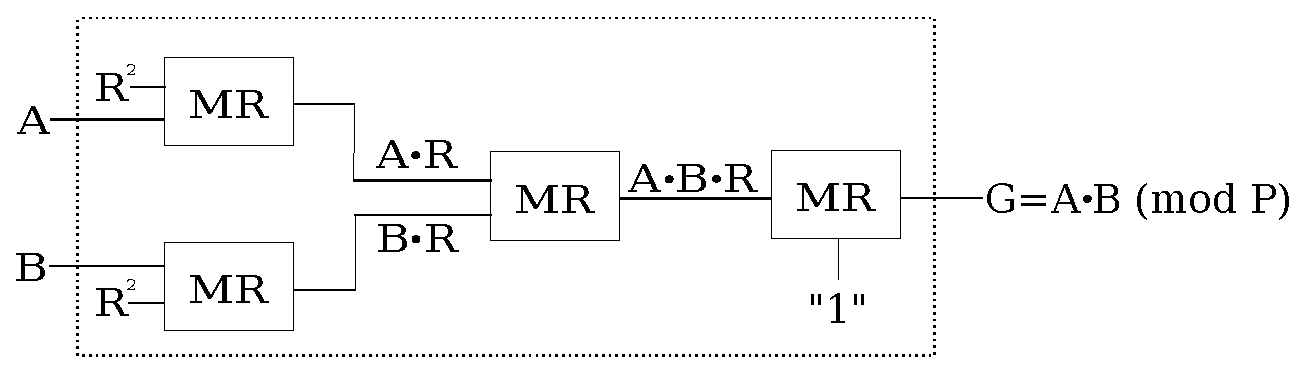
\includegraphics[scale=0.34]{new_mmcircuit}
  \caption{Montgomery multiplication.}
  \label{montfig}
  \end{figure}



\par Table~\ref{montmmsyn} provides the results for GBR on flattened
(bit-blasted) and  optimized Montgomery multipliers for the sequential
and parallel executions of Algorithm
\ref{multimon}. \textcolor{red}{The maximum  
memory consumption for sequential execution varies from 
66.7 MB for 64-bit operands to 11.3 GB for 571-bit operands.} 
% For most of these benchmarks the overhead is quite small than the
% reduction time for one bit except for the 233 and 409 bit
% multipliers. Therefore, we benefit from parallelizing the reduction
% process for these cases other than 283 and 409 bit multipliers.  
Our approach outperforms conventional explicit approaches except for
the case of 283 bit multiplier. 
% \textcolor{red}{Also, the reduction time for
% 283-bit circuit is more than 409-bit circuit. The reason is that 
% the bit-width of the multipliers is not the only factor controlling 
% the GBR time. The irreducible polynomial $P(x)$ also plays an
% important role in the designing of the multiplier and 
% consequently in the reduction as explained in \cite{cunxi:aspdac17}.} 

%%%%%%%%%%%%% Syn Mont Multipliers %%%%%%%%%%%%%%%%%%
%\iffalse
\begin{table}[H]
\centering
%\caption{Synthesized Mastrovito Multipliers (Time in seconds, \# of nodes, \# of redundant monomials in $k$)  (K = $10^3$, M = $10^6$)}
\caption{Montgomery Multipliers (Time in seconds); $k$ = Datapath Size, \#Gates = No. of gates, \#T = No. of threads, Time-Out = 30 hrs, (P): Parallel Execution, (S): Sequential Execution, K = $10^3$, M = $10^6$, PB: PolyBori, ZR: Algorithm~\ref{multimon}}
\label{montmmsyn}
\begin{tabular}{| c | c || c | c | c | c | c | c | c |} \hline
%\multirow{2}{*}{\textbf{Input}} & \multirow{2}{*}{\textbf{Abstraction}} & \multicolumn{3}{ c |}{\textbf{ZBDD reduction(ZR)}}  &  \multirow{2}{*}{\textbf{ZR improved}}\\ \cline{3-5}
% & &Building ZBDDs&Reduction&Total&\\ \hline
\multirow{2}{*}{$\boldsymbol{k}$}&\multirow{2}{*}{\textbf{\#Gates}}&\multirow{2}{*}{\textbf{F4~\cite{pruss:tcad}}}& \multirow{2}{*}{\textbf{\#T}}&\multirow{2}{*}{\textbf{~\cite{cunxi:aspdac17}(P)}}& \multicolumn{2}{ c |}{\textbf{PB}}&\multicolumn{2}{ c |}{\textbf{ZR}}\\ \cline{6-9}
&&&&&\textbf{(P)}&\textbf{(S)}&\textbf{(P)}&\textbf{(S)} \\ \hline
64 &9.5K&16.29&20&10.69&6.27&9.22& \textbf{3.75} & 8.37\\ \hline 
%96 &20.3K&&20&36.40&24.22& 22.0&\textbf{17.56} & 21.15\\ \hline 
128 &35K&621.90&20& 36.19&28.93&34.59&  \textbf{13.76}&24.73\\ \hline 
163 &56.5K&2,608.4&20&204.94 &167.73&335.2&  \textbf{141.68}&321.60\\ \hline 
233 &111K&385.92& 20&132.51& 119.77&99.36 &42.16&\textbf{31.88}\\ \hline
283 &165K&5,344& 20&\textbf{704.13}&1,194.2&2,078& 1,065.3&2,113\\ \hline
409 &340K&7,104& 10& 697.91&737.23& 722.1&303.91&\textbf{299.92}\\ \hline
571* &1.97M&TO&3&TO&CR&CR&\textbf{43,813}&99,042 \\ \hline
\end{tabular}
\end{table}
%\fi
%%%%%%%%%%%%%%%%%%%%%%%%%%%%%%%%%%%%%%%%%

\par Table \ref{montblockmm} presents the
statistics for Montgomery multipliers where the hierarchy of
Fig. \ref{montfig} for the blocks A, B, C, and D is made
available. The experiment first reduces the outputs of each individual
block modulo the gates of that block, and then reduces the primary
outputs modulo these four sets of remainders (ZBDDs), thus exploiting
the hierarchy of these circuits. Table~\ref{montblockmm} shows the time
for reduction of each block and the time for reducing the primary
outputs across the four blocks. The  time for reducing the primary
outputs across the hierarchical blocks in case of the F4
implementation is $<$1 second, and is not explicitly mentioned in the
table. The row labeled \textit{Total} presents the sum of the
computation time of 
reduction across these levels, and the maximum of the time to reduce
each MR block (as the reductions for the four blocks are independent
of each other and are parallelized). These results again demonstrate
the efficiency of our approach against explicit approaches.
% The datapath sizes of these circuits correspond to
% NIST-specification in cryptography with $k = 163,\dots,571$ bits.

\begin{table}[H]
\centering
% \caption{Montgomery Blocks(Time in seconds, Red. = time for reduction,
%   Coll. = time to reduce across the 4 levels.)}
\caption{Montgomery Blocks (Time in seconds); $k$ = Datapath Size, \#Gates = No. of gates, Time-Out = 30 hrs, 
Red. = time for reduction, Coll. = time to reduce across the 4 levels. 
% (P): Parallel Execution, (S): Sequential Execution, 
K = $10^3$, M = $10^6$, PB: PolyBori, ZR: Algorithm~\ref{multimon}}

\label{montblockmm}
\begin{tabular}{| c | c | c || c | c | c | c | c |} \hline
\multirow{2}{*}{$\boldsymbol{k}$}& \multirow{2}{*}{\textbf{\#Gates}}&\multirow{2}{*}{\textbf{Block}}& \multirow{2}{*}{\textbf{F4~\cite{pruss:tcad}}}  & \multicolumn{2}{ c |}{\textbf{PB}} &  \multicolumn{2}{ c |}{\textbf{ZR}} \\ \cline{5-8}
  & & & &Red. & Coll.  &Red. & Coll.  \\ \hline
\multirow{4}{*}{163} &33K &Block A & 25& 12 &\multirow{4}{*}{16} & 1 & \multirow{4}{*}{18}\\  \cline{2-5} \cline{7-7}
 & 33K&Block B &25 & 12 & & 1  &  \\  \cline{2-5} \cline{7-7}
 &85K&Block C &73 & 18 &&  7 &  \\  \cline{2-5} \cline{7-7}
 &32K&Block D &24 & 12 & & 1 & \\ \cline{2-8}
 &\multicolumn{2}{ c ||}{\textbf{Total}} & 73  &   \multicolumn{2}{ c |}{34} & \multicolumn{2}{ c |}{\textbf{25}}\\ \noalign{\hrule height 1.5pt}
\multirow{4}{*}{233}&55K&Block A  &142  & 32 & \multirow{4}{*}{5} & 0.14 & \multirow{4}{*}{4}\\  \cline{2-5} \cline{7-7}
 &55K& Block B &141 & 33 && 0.14  &  \\  \cline{2-5} \cline{7-7}
 &163K&Block C &408 & 34 & & 2.1  &  \\  \cline{2-5} \cline{7-7}
 &54K&Block D & 140& 32 && 0.13 & \\ \cline{2-8}
&\multicolumn{2}{ c ||}{\textbf{Total}}& 408  &   \multicolumn{2}{ c |}{39} & \multicolumn{2}{ c |}{\textbf{6.1}}\\ \noalign{\hrule height 1.5pt}
\multirow{4}{*}{283}&82K&Block A & 330 & 79 & \multirow{4}{*}{26} &24 & \multirow{4}{*}{90}\\  \cline{2-5} \cline{7-7}
&82K & Block B &329 & 78 && 23  &  \\  \cline{2-5} \cline{7-7}
&241K &Block C &883 & 173 &&  118 &  \\  \cline{2-5} \cline{7-7}
&81K &Block D &321 & 80 && 23 & \\ \cline{2-8}
&\multicolumn{2}{ c ||}{\textbf{Total}} & 883  &   \multicolumn{2}{ c |}{\textbf{199}} & \multicolumn{2}{ c |}{208}\\ \noalign{\hrule height 1.5pt}
\multirow{4}{*}{409}&168K&Block A & 1,322 & 177&\multirow{4}{*}{28} & 0.57 & \multirow{4}{*}{29}\\ \cline{2-5} \cline{7-7}
& 168K& Block B &1,335 &  175 &&  0.57 &  \\ \cline{2-5} \cline{7-7}
& 502K&Block C &4,471 & 192 &&  14 &  \\  \cline{2-5} \cline{7-7}
&168K &Block D &1,338 & 176 && 0.56 & \\ \cline{2-8}
&\multicolumn{2}{ c ||}{\textbf{Total}} & 4,471  &   \multicolumn{2}{ c |}{220} & \multicolumn{2}{ c |}{\textbf{43}}\\ \noalign{\hrule height 1.5pt}
\multirow{4}{*}{571}&330K&Block A &5,371 & 769 & \multirow{4}{*}{1,341} &321  & \multirow{4}{*}{1,412}\\  \cline{2-5} \cline{7-7}
&330K & Block B &5,421 & 747 && 332  &  \\ \cline{2-5} \cline{7-7}
 &980K&Block C &37,804 & 3,605 &&  3026 &  \\  \cline{2-5} \cline{7-7}
 &328K&Block D &5,539 & 751 && 338 & \\ \cline{2-8}
&\multicolumn{2}{ c ||}{\textbf{Total}}& 37,804  &   \multicolumn{2}{ c |}{4,946} & \multicolumn{2}{ c |}{\textbf{4,438}}\\ \noalign{\hrule height 1.5pt}


\end{tabular}
\end{table}


{\bf Equivalence Checking:} As a result of the GBR
$z_i\xrightarrow{G}_+ r_i$, the function implemented by each output
bit $z_i$ of the circuit is represented as a reduced, canonical,
Boolean polynomial in terms of the primary inputs, and by using a ZBDD.
Thus the equivalence of such vastly different arithmetic circuit
implementations (Mastrovito vs Montgomery) can be verified by testing
for the equality (isomorphism) of the corresponding ZBDD graphs. 


 %%%%%%%%% Point Addition Block D%%%%%%%%%%%%%%%%%%%%%%%%
\subsection{Point Addition over Elliptic Curves}
Point addition is an important operation required for the task of encryption, decryption 
and authentication in Elliptic Curve Cryptography (ECC). 
Modern approaches represent the points in projective
coordinate systems, {\it e.g.}, the L$\acute{o}$pez-Dahab (LD) projective coordinate \cite{eccld}, due to which the point addition 
operation can be implemented as polynomials in the field. 

\begin{Example}
{\it Consider point addition in L$\acute{o}$pez-Dahab (LD) projective coordinate. Given an elliptic curve: $Y^2 + XYZ = X^3Z + aX^2Z^2 + bZ^4$ over $\mathbb{F}_{2^k}$, where $X,Y,Z$ are $k$-bit vectors that are elements in $\mathbb{F}_{2^k}$ and similarly, $a, b$ are constants from the field. We represent point addition over the elliptic curve as ($X_3$, $Y_3$, $Z_3$) = ($X_1$, $Y_1$, $Z_1$) + ($X_2$, $Y_2$, $1$).  Then $X_3$, $Y_3$, $Z_3$ can be computed as follows:} 

\begin{align*}
&A = Y_2 \cdot Z_1^2 + Y_1  &&B = X_2 \cdot Z_1 + X_1 \\
&C = Z_1 \cdot B  &&D = B^2 \cdot(C + a Z_1^2) \\
&Z_3 = C^2 && E = A \cdot C  \\
&X_3 = A^2 + D + E &&F = X_3 + X_2 \cdot Z_3 \\
&G = X_3 + Y_2\cdot Z_3 && Y_3 = E\cdot F + Z_3 \cdot G \\
\end{align*}
\end{Example}

Each of the polynomials in the above design are implemented as a
(gate-level) logic block and are interconnected to obtain final
outputs $X_3,Y_3$ and $Z_3$. 

\begin{table}[H]
\centering
\caption{Point Addition Circuits (Time in seconds); $k$ = Datapath Size, \#Gates = No. of gates, Time-Out = 30 hrs, K = $10^3$, M = $10^6$,
PB: PolyBori, ZR: Algorithm~\ref{multimon}}
\label{pointadd}
\begin{tabular}{| c | c || c | c | c |} \hline
$\boldsymbol{k}$&\textbf{\#Gates}&\textbf{F4~\cite{pruss:tcad}}&\textbf{PB}&\textbf{ZR} \\ \hline
64&15.3K&1.78&3.32&\textbf{0.72} \\ \hline
128&64K&40.55&27.41&\textbf{6.03} \\ \hline
163&104K&130.24&57.57&\textbf{13.13} \\ \hline
233&139K&335.60&106.85&\textbf{19.62} \\ \hline
283&281K&1,787.96&273.53& \textbf{64.48}\\ \hline
409&423K&5,077.50&578.15& \textbf{115.20}\\ \hline
571&1.14M&48,162.29&CR&\textbf{725.95} \\ \hline
\end{tabular}
\end{table}

The word-level abstraction approach in~\cite{pruss:tcad} presents the
results for extracting  the above representation for each of
$A,B,\dots, X_3,Y_3,Z_3$ blocks. It first performs a bit-level
reduction for every output of each block (GBR $z_i\xrightarrow{G}_+
r_i$), and then a  bit-to-word substitution to derive an input-output
word-level representation for the circuit. Table~\ref{pointadd} shows
the comparison of the time required for bit-level reduction of outputs
$d_i$ of the block $D= B^2\cdot(C + aZ_1^2)$ as done
in~\cite{pruss:tcad} against our implementation. (Bit-level
reductions for other blocks take much less time than that for block
D.) This result demonstrates that our bit-level GBR implementation
is in many cases orders of magnitude faster than the F4-style
reduction of \cite{pruss:tcad}. Therefore our approach can replace the
F4-style bit-level GBR of \cite{pruss:tcad} and improve the overall
process of word-level abstraction of datapath designs.   

\subsection{Equivalence Checking of Sequential Galois Field Multipliers}
The designs discussed so far are combinational implementations of
polynomial computations of finite filed circuits. These designs use
the standard basis representation $\{1,\alpha,\alpha^2, \dots,
\alpha^{k-1}\}$ to model a $k$-bit data-word $Z$ in terms of its
constituent bits as $Z = z_0 + z_1 \alpha + z_2 \alpha^2 \cdots +
z_{k-1} \alpha^{k-1}$, with $\alpha$ being the primitive element for
that field $\mathbb{F}_{2^k}$. 

\par 
%The size of the multipliers presented in the above sections
%become prohibitively large as $k$ increases.  
There exists sequential
multipliers where $k$-bit inputs are loaded into $k$-bit registers,
and the $k$-bit result is available  after $k$ clock-cycle execution
of the machine. These multipliers use a {\it normal basis}
$\{\beta,\beta^{2},\beta^{4},\dots,\beta^{2^{k-1}}\}$ to  represent a
$k$-bit data-word $S$ in terms of its constituent bits as $S =
s_0\beta + s_1\beta^{2} + s_2\beta^{4} \cdots s_{k-1}\beta^{2^{k-1}}$,
with $\beta$ being the normal element. The relation between $\alpha$
and $\beta$ can be used to represent  the bits $z_i$ and $s_j$ in
terms of each other.  

% \par The Normal basis are more efficient when performing multiplication and 
% exponentiations. The exponentiation operation can be achieved by simple cyclic-shift of the input bits. 
% As multiplication is more complex than exponentiation, it is performed by constructing a binary-valued $\lambda$-matrix $M$.
% %and then performing $A\times M \times B^T$ for inputs $A$ and $B$. 
% If the  matrix $M$ satisfies the property that the number non-zero elements is $2k-1$ (for data-path size $k$), then the
% normal basis is called an optimal normal basis (ONB). ONB is desirable for the construction
% of finite field circuits.  

\par We perform equivalence checking between two different
architectures of {\it sequential multipliers with parallel output
  (SMPO)}, the Agnew-SMPO (AG-SMPO) by
G.B. Agnew~\cite{agnew1991implementation} and the RH-SMPO by
Reyhani-Masoleh and Hasan~\cite{RHmulti}. The values in the registers
for all intermediate states  in these multipliers are different
because they are based on two different mathematical principles.
However, the final state of the output registers (i.e. after $k$ clock
cycles) is the same as it is the result of the multiplication. In
order to perform equivalence checking, the circuits are unrolled
over $k$ time frames, and the GBR $s_i \xrightarrow{G}_+ r_i$ 
is performed to obtain a canonical $r_i$ ($G$ is the set of
polynomials for the unrolled circuit under RTTO). The ZBDDs for
respective $r_i$'s (for AG-SMPO and RH-SMPO) are compared to perform
equivalence check.    

% \par The authors in \cite{xiaojun:date15}\cite{xiaojun:phd} present an implicit unrolling approach for 
% sequential multipliers to derive a canonical word-level input-output relation. They present results for 
% two architectures of {\it sequential multipliers with parallel output (SMPO)} based on different 
% mathematical principles, the Agnew-SMPO (AG-SMPO) by G.B. Agnew~\cite{agnew1991implementation}
% and the RH-SMPO by Reyhani-Masoleh and Hasan~\cite{RHmulti}. 

%\par We perform the GBR $s_i \xrightarrow{G}_+ r_i$ for each output bit $s_i$ of the $k$-cycle unrolled 
% multipliers to obtain a canonical $r_i$. The $r_i$ can then be used to perform an equivalence check between the
% two architectures. 
Tables \ref{rhsmpo} and \ref{agsmpo} present the run-time of our
implementation for performing these reductions on RH-SMPO and AG-SMPO
architectures respectively, when compared with the approach presented
in \cite{pruss:tcad} and PolyBori. 
%Although normal bases exist for every $k$, optimal normal bases (ONB)
%do not. There are also different types of ONB. The values of $k$ in
%the tables correspond to Type-II ONB. For more details and a list of
%ONB field size, reader can refer to~\cite{gao:phd_normal_basis}. 
The results show that our implementation is about an order of
magnitude faster than PolyBori and multiple orders of magnitude faster
than the  explicit approach of~\cite{pruss:tcad}.
% The bit-widths in table are
% such that the corresponding normal basis are ONB. Our verification technique is multiple orders of magnitude faster than 
% that of~\cite{pruss:tcad} and an order of magnitude faster than the PolyBori.

\begin{table}[H]
\centering
\caption{RH-SMPO Multipliers \textcolor{red}{(Time in seconds)}; $k$ = Datapath Size, \#Gates = No. of gates, Time-Out = 30 hrs, K = $10^3$,
PB: PolyBori, ZR: Algorithm~\ref{multimon}}
\label{rhsmpo}
\begin{tabular}{| c | c | c | c | c | c | c | c | c |} \hline
$\boldsymbol{k=}$&65&81&89&131&173&233&281&410 \\ \hline
\textbf{\#Gates} & 13.6K&21.4K & 25.9K& 55.9K &96.5K&177K&258K&546K\\ \hhline{|=|=|=|=|=|=|=|=|=|}
\textbf{F4\cite{pruss:tcad}} &9.02 &26.65 & 42.46&294.7&874.3&3,404&7,328&23,610 \\ \hline
% \textbf{F4\cite{pruss:tcad}}   & 8.56&22.2 & 37.1&259.5&838.5&3,009&7566&23,610 \\ \hline %with bogus primitive polynomial
\textbf{PB}  &3.65 &6.07 & 7.42&28.22 &47.16&116.63&199.32&637.69\\ \hline
\textbf{ZR}  & \textbf{0.42}& \textbf{0.80}&\textbf{1.01} & \textbf{3.03}&\textbf{3.53}&
\textbf{8.12}&\textbf{13.27}&\textbf{52.09}\\ \hline
\end{tabular}
\end{table}

\begin{table}[H]
\centering
\caption{AG-SMPO Multipliers \textcolor{red}{(Time in seconds)}; $k$ = Datapath Size, \#Gates = No. of gates, Time-Out = 30 hrs, K = $10^3$,
PB: PolyBori, ZR: Algorithm~\ref{multimon}}
\label{agsmpo}
\begin{tabular}{| c | c | c | c | c | c | c | c | c |} \hline
$\boldsymbol{k=}$&65&81&89&131&173&233&281&410 \\ \hline
\textbf{\#Gates} &12.5K & 19.5K&23.6K&51.2K&89.4K&162K&236K&503K \\ \hhline{|=|=|=|=|=|=|=|=|=|}
\textbf{F4\cite{pruss:tcad}} &8.34 &20.46 &33.2&221.4&754.1&2,655&5,569&21,938\\ \hline
% \textbf{F4\cite{pruss:tcad}}  & 8.15& 19.18&29.1 &200.9&665.7&2,387&6,516&21,938 \\ \hline %with bogus primitive polynomial
\textbf{PB} &3.11 & 6.82& 9.21& 20.15&44.37&107.12&187.77&578.61\\ \hline
\textbf{ZR} &\textbf{0.44} &\textbf{0.77} &\textbf{0.91}& \textbf{2.51}&\textbf{3.39}&
\textbf{7.8}&\textbf{12.63}&\textbf{43.78}\\ \hline
\end{tabular}
\end{table}

% \begin{table}[H]
% \centering
% \caption{RH-SMPO Multipliers; $k$ = Datapath Size, \#Gates = No. of gates, Time-Out = 30 hrs, K = $10^3$,
% PB: PolyBori, ZR: Algorithm~\ref{multimon}}
% \label{rhsmpo}
% \begin{tabular}{| c | c | c | c | c | c | c | c | c | c | c |} \hline
% $\boldsymbol{k}$&33&51&65&81&89&131&173&233&281&410 \\ \hline
% \#Gates & 3.5K&8.5K & 13.6K&21.4K & 25.9K& 55.9K &96.5K&177K&258K&546K\\ \hhline{|=|=|=|=|=|=|=|=|=|=|=|}
% \cite{pruss:tcad} & 0.56& 3.3&9.02 &26.65 & 42.46&294.7&874.3&3,404&7,328& \\ \hline
% \cite{pruss:tcad} &0.88 &3.3 & 8.56&22.2 & 37.1&259.5&838.5&3,009&7566&23,610 \\ \hline %with bogus primitive polynomial
% PB &0.58 &1.96 &3.65 &6.07 & 7.42&28.22 &47.16&116.63&199.32&637.69\\ \hline
% ZR &\textbf{0.10} & \textbf{0.28}& \textbf{0.42}& \textbf{0.80}&\textbf{1.01} & \textbf{3.03}&\textbf{3.53}&
% \textbf{8.12}&\textbf{13.27}&\textbf{52.09}\\ \hline
% \end{tabular}
% \end{table}

% \begin{table}[H]
% \centering
% \caption{AG-SMPO Multipliers; $k$ = Datapath Size, \#Gates = No. of gates, Time-Out = 30 hrs, K = $10^3$,
% PB: PolyBori, ZR: Algorithm~\ref{multimon}}
% \label{agsmpo}
% \begin{tabular}{| c | c | c | c | c | c | c | c | c | c | c |} \hline
% $\boldsymbol{k}$&33&51&65&81&89&131&173&233&281&410 \\ \hline
% \#Gates &3.2K&7.7K&12.5K & 19.5K&23.6K&51.2K&89.4K&162K&236K&503K \\ \hhline{|=|=|=|=|=|=|=|=|=|=|=|}
% \cite{pruss:tcad} & 0.48& 2.78&8.34 &20.46 &33.2&221.4&754.1&2,655&5,569&\\ \hline
% \cite{pruss:tcad} &0.48 &2.76 & 8.15& 19.18&29.1 &200.9&665.7&2,387&6,516&21,938 \\ \hline %with bogus primitive polynomial
% PB & 0.52& 1.74&3.11 & 6.82& 9.21& 20.15&44.37&107.12&187.77&578.61\\ \hline
% ZR & \textbf{0.07}&\textbf{0.24} &\textbf{0.44} &\textbf{0.77} &\textbf{0.91}& \textbf{2.51}&\textbf{3.39}&
% \textbf{7.8}&\textbf{12.63}&\textbf{43.78}\\ \hline
% \end{tabular}
% \end{table}

% \begin{Example}
% {\it Consider a 3-bit RH-SMPO multiplier with output bits $\{r_2,r_1,r_0\}$ and input bits $\{p_2,p_1,p_0\}\{q_2,q_1,q_0\}$. 
% The multiplier performs the operation $R=P\cdot Q$, where $R=r_0\cdot \beta + r_1\cdot \beta^2 + r_2\cdot \beta^4$, 
% $P=p_0\cdot \beta + p_1\cdot \beta^2 + p_2\cdot \beta^4$ and $Q=q_0\cdot \beta +q_1\cdot \beta^2 + q_2\cdot \beta^4$. 
% Also consider a Mastrovito multiplier performing the operation $Z=A\cdot B$ with $Z=z_0\cdot  + z_1 \alpha + z_2\cdot \alpha^2$,
%  $A=a_0\cdot  + a_1 \alpha + a_2\cdot \alpha^2$ and $B=b_0  + b_1\cdot \alpha + b_2\cdot \alpha^2$ where $\{z_2,z_1,z_0\}$ and 
%  $\{a_2,a_1,a_0,b_2,b_1,b_0\}$ being the output and input bits respectively. The normal element $\beta$ in terms of standard basis 
%  element is $\beta = \alpha^3$. The primitive polynomial used in the design of Mastrovito multiplier is $P=X^3+X+1$ and $\alpha$ is the 
%  root of this polynomial.
%  \par The RH-SMPO multiplier output $R$ can be written in the notations of standard basis 
%  as $R = r_0\cdot \alpha^3 + r_1\cdot \alpha^6 + r_2\cdot \alpha^{12} = (r_0 + r_1 + r_2) + (r_0 + r_2)\cdot \alpha + (r_1 + r_2)\cdot \alpha^2$ using $\beta = \alpha^3$ and $\alpha^3 = \alpha +1$. Similarly, $P = (p_0 + p_1 + p_2) + (p_0 + p_2)\cdot \alpha + (p_1 + p_2)\cdot \alpha^2$ and $Q = (q_0 + q_1 + q_2) + (q_0 + q_2)\cdot \alpha + (q_1 + q_2)\cdot \alpha^2$. Therefore, }
% \begin{align*}
% & z_0 = r_0 + r_1 + r_2; ~~ z_1 = r_0 + r_2; ~~ z_2 = r_1 + r_2; \\
% & a_0 = p_0 + p_1 + p_2; ~~ a_1 = p_0 + p_2; ~~ a_2 = p_1 + p_2; \\
% & b_0 = q_0 + q_1 + q_2; ~~ b_1 = q_0 + q_2; ~~ b_2 = q_1 + q_2;
% \end{align*}
% {\it Solving for $p_i$ and $q_i$ in terms of $a_i$ and $b_i$ respectively,}
% \begin{align*}
% & p_0 = a_0 + a_2; ~~ p_1 = a_0 + a_1; ~~ p_2 = a_0 + a_1 + a_2; \\
% & q_0 = b_0 + b_2; ~~ q_1 = b_0 + b_1; ~~ q_2 = b_0 + b_1 + b_2;
% \end{align*}
% {\it Performing a bit-level reduction on $r_0,r_1$ and $r_2$ results in the following remainders,}
% \begin{align*}
% & r_0 = p_1\cdot q_0 + p_0\cdot q_1 + p_2\cdot q_1 + p_1\cdot q_2 + p_2\cdot q_2 \\
% & r_1 = p_0\cdot q_0 + p_2\cdot q_0 + p_2\cdot q_1 + p_0\cdot q_2 + p_1\cdot q_2 \\
% & r_2 = p_1\cdot q_0 + p_2\cdot q_0 + p_0\cdot q_1 + p_1\cdot q_1 + p_0\cdot q_2
% \end{align*}
% {\it Using $z_0 = r_0 + r_1 + r_2$, we get $z_0 = p_0\cdot q_0 + p_1\cdot q_1 + p_2\cdot q_2$. 
% Substituting $\{p_i,q_i\}$ in terms of $\{a_i,b_i\}$ results in $z_0 = a_0\cdot b_0 + a_1\cdot b_2 + a_2\cdot b_1$,
% which is also the remainder if we reduce the $z_0$ bit of the Mastrovito multiplier 
% modulo the polynomials of the gates of the circuit.
% }

% \end{Example}

% \begin{table}[H]
% \centering
% \caption{RH-SMPO Multipliers; k = Datapath Size, \#Gates = No. of gates, Time-Out = 30 hrs, K = $10^3$}
% \label{rhsmpo}
% \begin{tabular}{| c | c | c | c | c | c | c |} \hline
% \textbf{k}&33&51&65&81&89&99 \\ \hline
% \#Gates & 3.5K&8.5K & 13.6K&21.4K & 25.9K& 32K\\ \hline
% \cite{xiaojun:date15} & 112.6& 1,129&5,243 &20,724 &36,096 &67,021 \\ \hline
% PB & 0.59& 2.02&3.10 &5.99 &7.72 &13.26 \\ \hline
% ZR &\textbf{0.10} & \textbf{0.26}& \textbf{0.48}& \textbf{0.84}&\textbf{1.08} & \textbf{1.48}\\ \hline
% \end{tabular}
% \end{table}

% \begin{table}[H]
% \centering
% \caption{AG-SMPO Multipliers; k = Datapath Size, \#Gates = No. of gates, Time-Out = 30 hrs, K = $10^3$}
% \label{agsmpo}
% \begin{tabular}{| c | c | c | c | c | c |} \hline
% \textbf{k}&36&66&82&89&100 \\ \hline
% \#Gates &3.8K&13K&20K & 23.6K&29.8K \\ \hline
% \cite{xiaojun:date15} & 113& 3,673& 15,117& 28,986& 50,692\\ \hline
% PB &0.48 & 2.84& 6.93&7.29 & 9.91 \\ \hline
% ZR & \textbf{0.10}&\textbf{0.46} &\textbf{0.76} &\textbf{0.95} &\textbf{1.30} \\ \hline
% \end{tabular}
% \end{table}


\subsection{Limitations of our approach: Integer arithmetic circuits}
% \par {\bf Integer Multiplication:} When performing reduction on
% integer multiplication benchmarks, a large number of non-linear  %
% monomials are generated that can be canceled early in the reduction
% process by employing a word-level approach unlike  % our bit-level
% reduction approach.  % The polynomial algebra model is not suitable
% for random logic (synthesized) circuits, where AIG-based reduction
% makes verification efficient. This model is beneficial for custom
% designed arithmetic circuits, where AIGs/SAT fail. 
\textcolor{red}{
The GBR approach presented in the previous section, although
applicable to integer arithmetic circuits, is not computationally
feasible for their verification. 
%The logical cones of output variables in integer
%arithmetic circuits have a lot of logic sharing (common subexpressions) and generate a
%large number of non-linear terms. 
We evaluated  our technique on integer arithmetic multiplier
circuits, which showed an  exponential increase in verification time
$w.r.t.$ the circuit size. This is because our approach reduces 
each primary output bit independently, and does not consider the logic
sharing among different primary outputs. As a result, a large number
of monomials are generated during reduction that are common to 
multiple primary outputs. This effect of logic sharing cannot be
exploited in GBR when each primary output bit is reduced
independently. 
For example, the ZBDD-based bit-level GBR for a 7x7 integer
multiplier reveals that when reducing the $z_{13}$ bit (MSB) and
the $z_{12}$ bit independently, the maximum number of monomials
encountered ($i.e.$ during $z_{13} \xrightarrow{G}_+ r_{13}$ and
$z_{12} \xrightarrow{G}_+ r_{12}$) are 429,889 and 897,955,
respectively.  However, the modulo-2 sum (XOR) of these ZBDDs contains
only 789,604 monomials  (during the modulo-2 sum common monomials
cancel out) as opposed to 1,327,844 (= 429,889 + 897,955).
A word-level reduction approach (such as those of
\cite{ciesielski:dac2015} and \cite{rolf:date16}) may cancel such
common non-linear terms early in the reduction process and avoid
intermediate blow-up in the number of monomials. This is shown below.
%This  
%implies that even an implicit data-structure
%cannot accommodate the large number of non-linear terms
%that result in intermediate expression swell.
% Performing a detailed analysis reveals that for
% integer arithmetic datapath circuits, a bit-level reduction is {\it
%   not sufficient} for verification efficiency, and a word-level
% approach is required. %, such as the ones presented in 
}

\begin{figure}[hbt]
\centering
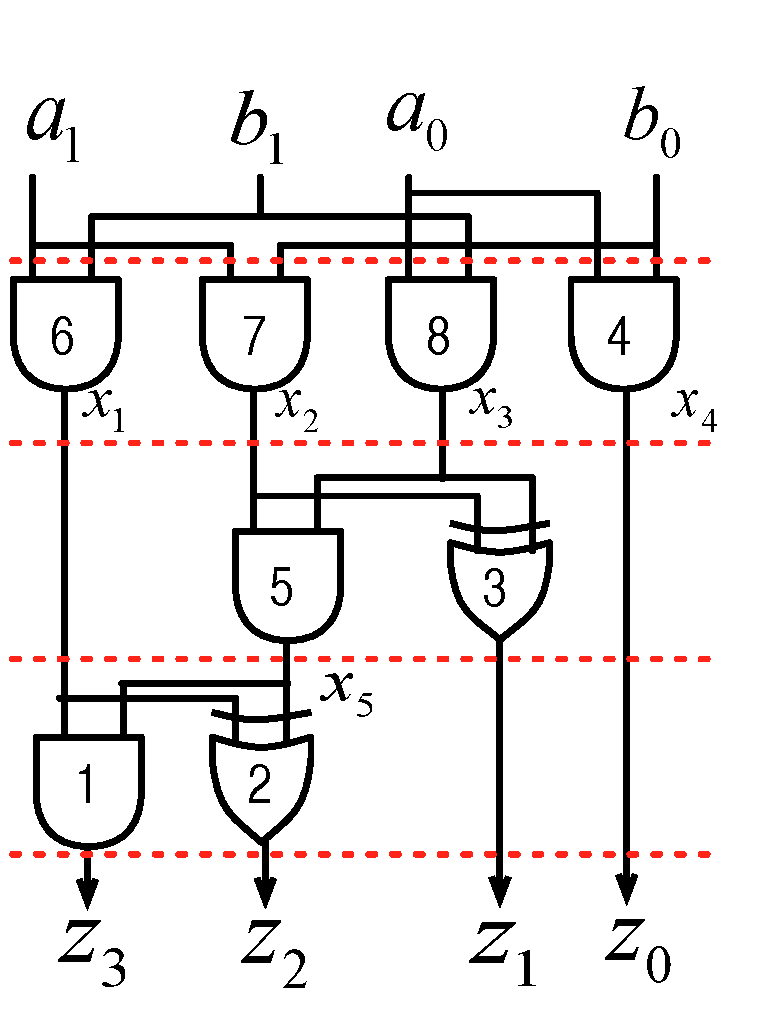
\includegraphics[scale=0.4]{2-bit-mult.pdf}
\caption{Integer multiplier circuit}
\label{intmult}
\end{figure}

%\textcolor{red}{ A better 
%approach would be to perform a word-level reduction similar to
%the following example.
%}

\textcolor{red}{Consider the integer multiplier circuit given in
  Fig. \ref{intmult}. A 
word-level approach would model the output word as 
$Z = z_0 + 2z_1 + 4 z_2 + 8 z_3$, and perform the reduction
$Z\xrightarrow{G}_+R$ across the reverse topological levels (RTTO) 
depicted in the figure. The polynomials of the circuit are:} 

\textcolor{red}{\begin{align*}
z_0 &= x_4\\
z_1 &= x_2 + x_3 - 2x_2x_3\\
z_2 &= x_1 + x_5 - 2 x_1 x_5\\
    &= x_1 + x_2x_3 - 2x_1x_2x_3\\
z_3 &= x_1x_5 = x_1x_2x_3
\end{align*}}

\textcolor{red}{Here $+$ denotes addition over integers. The reduction
  of the word-level expression $8z_3 + 4z_2+2z_1+z_0$ in $Z$ cancels out the
  common nonlinear monomials to control intermediate monomial explosion: }

\textcolor{red}{\begin{align*}
Z &= 8z_3 + 4z_2+2z_1+z_0\\
  &=\underline{8x_1x_2x_3} + (4x_1 + \underbrace{4x_2x_3} -
  \underline{8x_1x_2x_3})\\
  & + (2x_2+2x_3-\underbrace{4x_2x_3}_{}) + x_4\\
  &=\textcolor{red}{4x_1 + 2x_2 + 2x_3 + x_4}
\end{align*}
}

\textcolor{red}{A purely
bit-level GBR approach is thus not suitable for integer arithmetic
circuits. However, this is not a limitation of our algorithms and
implementations, but rather an issue of the capability of bit-level
versus word-level models. Integrating the implicit data structure with
a word-level representation may yield better results for
such applications.} 

%% This modulo-2 sum indicates that reducing all the outputs simultaneously results 
%% in monomials that can cancel each other. Therefore, verification of integer multipliers require a word-level
%% decision procedure, as given in \cite{ciesielski:dac2015}
%% \cite{rolf:date16}, that accounts for the cancellation of these
%% monomials across multiple bits in one word-level expression whereas a pure bit-level reduction
%% is not sufficient to solve the problem. The experiment suggests that for integer 
%% arithmetic multipliers, 



% The reduction times for small integer arithmetic array multipliers are
% presented in Table \ref{intmm}. There is an 8x increase in time when
% moving from $n-1$ datapath size to $n$-bits, which is an exponential
% increase. Performing detailed analysis of a 7x7 multiplier reveals
% that, when reducing the $z_{13}$ bit (MSB) and $z_{12}$ bit of this
% circuit, the maximum number of monomials encountered are 429,889 and
% 897,955. Of these, 269,120 monomials are {\it common to both output
%   bits}. This implies that integer multipliers require a word-level
% decision procedure, as given in \cite{ciesielski:dac2015}
% \cite{rolf:date16}, that account for the cancellation of these
% monomials across multiple bits in one word-level expression. Our
% results show that bit-level techniques cannot efficiently verify
% integer arithmetic circuits, but are very efficient for finite-field
% arithmetic circuits. 

% \begin{table}[H]
% \centering
% \caption{Integer Array Multipliers (Time in seconds)}
% \label{intmm}
% \begin{tabular}{| c | c | c | c | c |} \hline
% \textbf{Datapath}&7&8&9&10 \\ \hline
% \textbf{Time}& 1& 8 &66&478 \\ \hline
% \end{tabular}
% \end{table}


%%%%%%%%%%%%%%%%%%%%%%%%%%%%%%%%%%%%%%%%%%%%%%%%%%%%%%%%

\section{Conclusion} \label{sec:conc}
This paper has presented an approach for formal verification of 
datapath circuits by deriving a canonical polynomial representation
for each output bit $z_i$ of a circuit in terms of the primary inputs
using Gr\"obner basis reduction. The gates of the circuit $C$ are
modeled as a set of polynomials $G$ over $\mathbb{F}_2$ where the
variables are the nets of the circuit. An order on the variables is
derived from the topology of the circuit, and a $lex$ term order
(RTTO) is imposed on the polynomials. RTTO renders the set $G$ a
Gr\"obner basis  itself. The reduction $z_i\xrightarrow{G}_+ r_i$
results in a canonical remainder $r_i$ for  each output $z_i$. 
%The complexity of computing the
%Gr\"obner basis can be avoided by deriving a term order from th
%topology of the circuit, which renders this set of polynomials itself
%as  a Gr\"obner basis. 
\par The polynomials in the set $G$ are Boolean polynomials that can 
be construed as unate cube sets. The unate cube set algebra prowess of
ZBDDs is exploited to represent the polynomials implicitly. We show
that RTTO imposes a special structure on the ZBDDs, where
subexpressions for leading monomials and quotients of the division are
readily visible as subgraphs in the ZBDD. We take further advantage of
this data structure to improve the classical \Grobner basis reduction 
method that relies on canceling only 1 monomial in every iteration
of division. Our approach cancels multiple monomials in each step of
division and generates fewer terms, thus speeding up the reduction. 
We have performed experiments with various finite field circuits used in
cryptography. Our approach achieves significant improvement over
recent approaches: the F4-style reduction, a parallelized approach for
reduction, and PolyBori. 
% The  efficiency of our approach is demonstrated by completing the
% reduction for up to 571-bit modulo Montgomery multipliers in the allotted time,
% and significant improvement is achieved over the F4-style reduction,
% parallelized reductions and  PolyBori based techniques. 

As part of our future work, we are pursuing investigations to
discover a pseudo-Boolean ``word-level signature'' of the GBR
$Z\xrightarrow{G}_+R$, that could be integrated with implicit
representations for integer arithmetic circuits.   

\par \textbf{Acknowledgment:} The authors wish to thank Cunxi Yu of
the University of Massachusetts, Amherst for assistance with
logic synthesis and optimization of some of the benchmarks used in the
experiments.  
%\end{document} 
%%%%%%%%% Mas571 Multipliers %%%%%%%%%%%%%%%%%%%%%%%%
\iffalse
\begin{table}[H]
\centering
\caption{Structured 571 bit Multipliers (Time in seconds);  \#Gates = No. of gates, \#T = No. of threads, Time-Out = 1 day, (P): Parallelization, (WP): Without Parallelization, K = $10^3$}
\label{montmmsyn}
\begin{tabular}{| c | c | c | c | c | c | c | c |} \hline
\textbf{Architecture} & \textbf{\#Gates}&\textbf{F4} & \textbf{\#T} & \textbf{~\cite{cunxi:aspdac17}(P)} & \textbf{PB} & \textbf{ZR(P)} & \textbf{ZR(WP)} \\ \hline
Mastrovito&1,600K&TO&3&5,331&CR&2,126.65&566 \\ \hline
Montgomery&1,970K&TO&3&TO&CR&43,813&TO \\ \hline
\end{tabular}
\end{table}
\fi
%%%%%%%%%%%%%%%%%%%%%%%%%%%%%%%%%%%%%%%%%
%%%%%%%%% OLD TABLES%%%%%%%%%%%%%%%%%%%%%%%%%%
%%%%%%%%%%%%%%%%%%%%%%%%%%%%%%%%%%%%%%%%%
%%%%%%%%%%%%%%%%%%%%%%%%%%%%%%%%%%%%%%%%%
\iffalse
\begin{table*}
\centering
\caption{Mastrovito Multipliers (Time in seconds, \# of nodes, \# of redundant monomials in $k$)  (K = $10^3$, M = $10^6$)}
\label{masmm}
\begin{tabular}{| c | c | c | c | c | c | c |} \hline
%\multirow{2}{*}{\textbf{Input}} & \multirow{2}{*}{\textbf{Abstraction}} & \multicolumn{3}{ c |}{\textbf{ZBDD reduction(ZR)}}  &  \multirow{2}{*}{\textbf{ZR improved}}\\ \cline{3-5}
% & &Building ZBDDs&Reduction&Total&\\ \hline
\textbf{Datapath(k)}&\textbf{\# of Gates} & \textbf{F4} & \textbf{PB} &\textbf{ZR} & \textbf{MN/MR} & \textbf{CS}\\ \hline
163 &153K& 1,443s &70s& \textbf{10s} & 811/765 & 153K\\ \hline 
233 &167K& 1,913s &105s& \textbf{14s} & 772/699& 167K\\ \hline
283 &399K& 11,116s &316s& \textbf{45s} & 1,413/1,402&400K\\ \hline
409 &508K& 17,848s &596s& \textbf{75s} & 1,313/1,227&508K\\ \hline
571 &1.6M& 192,032s &CR& \textbf{616s} & 2,849/2,840&1.6M\\ \hline 


\end{tabular}
\end{table*}
\fi

\iffalse
\begin{table*}
\centering
\caption{Montgomery Flat Multipliers (Time in seconds, \# of nodes in $k$, \# of redundant monomials in $k$) (K = $10^3$, M = $10^6$, B = $10^9$)}
\label{montmm}
\begin{tabular}{| c | c | c | c | c | c | c |} \hline
%\multirow{2}{*}{\textbf{Input Bit-width}} & \multirow{2}{*}{\textbf{Abstraction}} & \multicolumn{3}{ c |}{\textbf{ZBDD reduction(ZR)}}  &  \multirow{2}{*}{\textbf{ZR improved}} \\ \cline{3-5}
% & &Building ZBDDs&Reduction&Total& \\ \hline
\textbf{Datapath(k)}&\textbf{\# of Gates} & \textbf{F4} & \textbf{PB} &\textbf{ZR} & \textbf{MN/MR} & \textbf{CS}\\ \hline
163 & 184K&6,897s &\textbf{9294s}&9,595 & 39.4K/765 & 823M\\ \hline 
233 & 329K&63,805s &1749s&\textbf{1,452s}&4.4K/699 & 186M\\ \hline
283 & 488K&TO &\textbf{127,096s}& 247,837s &117K/1.4K &8.7B\\ \hline
409 & 1.0M&TO & \textbf{19,679s}& 32,226s &9.5K/1.2K &1.4B\\ \hline
571 & 1.97M&TO &CR& \textbf{128,464s}& TO/2.9K & TO\\ \hline 

\end{tabular}
\end{table*}
\fi

\iffalse
\begin{table*}
\centering
\caption{Montgomery Blocks(Max Nodes/Remainder)  (K = $10^3$, M = $10^6$)}
\label{montblockstats}
\begin{tabular}{| c | c | c | c | c | c | c |} \hline
\textbf{Datapath(k)/Block} &&  \textbf{163} & \textbf{233} &\textbf{283} & \textbf{409} & \textbf{571} \\ \hline
\multirow{2}{*}{Block A} &MN/MR&64/9&10/5&155/10&11/5& 296/9\\ \cline{2-7}
& CS&301K & 98K& 2.3M & 345K & 17M\\ \hline
\multirow{2}{*}{Block B} &MN/MR&64/9&10/5&155/10&11/5& 296/9\\ \cline{2-7}
& CS&301K & 98K& 2.3M & 345K & 17M\\ \hline
\multirow{2}{*}{Block C} &MN/MR&3.2K/3.2K&705/701&13K/10K&1.2K/1.2K& 83K/82K\\ \cline{2-7}
& CS&301K & 98K& 2.3M & 345K & 17M\\ \hline
\multirow{2}{*}{Block D} &MN/MR&112/58&12/7&292/147&14/8& 578/291\\ \cline{2-7}
& CS&301K & 98K& 2.3M & 345K & 17M\\ \hline
\multirow{2}{*}{Collapse} &MN/MR&18K/765&1.5K/699&42K/1.4K&3K/1.2K& 167K/2.8K\\ \cline{2-7}
& CS& 1.8M& 321K & 12M&1.3M &96M \\ \hline
\end{tabular}
\end{table*}
\fi
%&&&&&&&&&& \\ \hline
%%%%%%%%%%%%%%%%%%%%%%%%%%%%%%%%%%%%%%%%%
%%%%%%%%%OLD TABLES END%%%%%%%%%%%%%%%%%%%%%%%%
%%%%%%%%%%%%%%%%%%%%%%%%%%%%%%%%%%%%%%%%%
%%%%%%%%%%%%%%%%%%%%%%%%%%%%%%%%%%%%%%%%%




\iffalse
\begin{table}
\centering
\caption{Integer Array Multipliers (Time in seconds)}
\label{intmm}
\begin{tabular}{| c | c | c | c | c |} \hline
\textbf{Datapath}&7&8&9&10 \\ \hline
\textbf{Time}& 1& 8 &66&478 \\ \hline
\end{tabular}
\end{table}

\fi

%%%%%%%%%%%%%%%%%% ENDS HERE %%%%%%%%%%%%%%%%%
\iffalse

\begin{table}
\centering
\caption{Montgomery Blocks(Time in seconds)}
\begin{tabular}{| c | c | c | c | c | c | c | c | c | c | c | c | c | c | c | c | } \hline
\multirow{2}{*}{\textbf{Input/Blocks}} & \multicolumn{3}{ c |}{\textbf{163}} & \multicolumn{3}{ c |}{\textbf{233}} & \multicolumn{3}{ c |}{\textbf{283}} & \multicolumn{3}{ c |}{\textbf{409}} & \multicolumn{3}{ c |}{\textbf{571}} \\ \cline{2-11}
&ABS&PB&ZR&ABS&PB&ZR&ABS&PB&ZR&ABS&PB&ZR&ABS&PB&ZR  \\ \hline
Block A &25&1&142&$<1$&330&28&1,322&$<1$&5,371&725 &&&&&\\ \hline
Block B &25&1&141&$<1$&329&29&1,335&$<1$&5,421&752 &&&&&\\ \hline
Block C &73&12&408&13&883&254&4,471&117&37,804&4,164 &&&&&\\ \hline
Block D &24&1&140&$<1$&321&30&1,338&$<1$&5,539&747 &&&&&\\ \hline
Collapse &$<1$&33&$<1$&9&$<1$&158&$<1$&58&$<1$&1,516 &&&&&\\ \hline 
Total &&&&&&&&&& &&&&&\\ \hline
\end{tabular}
\end{table}
 \fi

